\section{Overview}

This section provides a short overview of the developed system functionality and its components. In it will be described the selected EtherCAT library, ROS implementation structure, and developed mechanical setup. 

\subsection{EtherCAT library}

Various libraries for interfacing with the EtherCAT network stack are available. 

\begin{table}[H]
	\centering
	\begin{tabular}{|c|p{6cm}|}
		\hline
		\textbf{Name} & \textbf{Description} \\
		\hline
		Simple Open EtherCAT Master &  \\
		\hline
		EcMaster &  \\
		\hline
		EtherLab &  \\
		\hline
	\end{tabular}
	\caption{EtherCAT libraries}
	\label{tab:ethercat_libraries}
\end{table}

Besides the libraries listed in table \ref{tab:ethercat_libraries} several manufacturer implementations also exist.
They were avoided as they are usually not open-sourced and are mostly applicable to each manufacturers devices, although they in some cases can be used for other devices too. 

It was chosen to rely on the SOEM implementation. It is open-sourced under the GPLv2 license and has been stable for multiple years. 
Other projects such as \textcolor{red}{EXAMPLES PLEASE} have also implemented this library, providing some evidence that it is possible. 

When initializing the protocol it is required to elevate the capability set of the executable. 
This is due to it being a layer-2 and requiring access to a raw networking socket. 
Capability escalation is handled through a helper application, \textit{ethercat\_grant} \textcolor{red}{LINK PLEASE}. 

\subsection{ROS interfaces package}

To communicate within the ROS network some custom message and service type were created. 

\lstset{style=rosdef}
\begin{lstlisting}[caption=Parameter message type,label=lst:ros_interface_msg_parameter]
int16 index
int16 subindex
int8 type
int64 value

int8 UINT8=0
int8 INT8=1
int8 UINT16=2
int8 INT16=3
int8 UINT32=4
int8 INT32=5
int8 UINT64=6
int8 INT64=7
\end{lstlisting}

The parameter message defines int8 types for determining the type of each parameter value at runtime.
This is used to easily know which typecast to apply upon receiving as parameters can be a variety of types.

\begin{lstlisting}[caption=NetworkCtrl service type,label=lst:ros_interface_srv_networkctrl]
int8 action

int8 START=0
int8 STOP=1
---
int8 result
string msg

int8 ERROR=0
int8 SUCCESS=1
\end{lstlisting}

\begin{lstlisting}[caption=GetParameters service type,label=lst:ros_interface_srv_getparameters]
int64 slave_index
---
ecat_interfaces/Parameter[] parameters
bool success
string msg
\end{lstlisting}

\begin{lstlisting}[caption=SetParameters service type,label=lst:ros_interface_srv_setparameters]
int64 slave_index
ecat_interfaces/Parameter[] parameters
---
bool success
string msg
\end{lstlisting}

\begin{lstlisting}[caption=ExecuteMove action type,label=lst:ros_interface_action_executemove]
int64[] time_data_ns
int64[] position_data_um
uint64 feedback_chunk_size
---
string msg
---
int64[] time_data_ns
int64[] position_data_um
\end{lstlisting}

\subsection{ROS network server}

To manage the EtherCAT network inside ROS2, a server node was developed specifically for this. 
The node presents services on the ROS network for starting and stopping the EtherCAT network, as well as provides a ROS action through which moves can be executed. 
The action returns feedback during the move. 
Due to the relatively fast loop times that can be achieved the action also provides a parameter for chunking feedback instead of returning it on each cycle. 
This was found to be necessary when communicating with the developed Python user interface to avoid dropping feedback values. 

\begin{figure}[H]
	\centering
	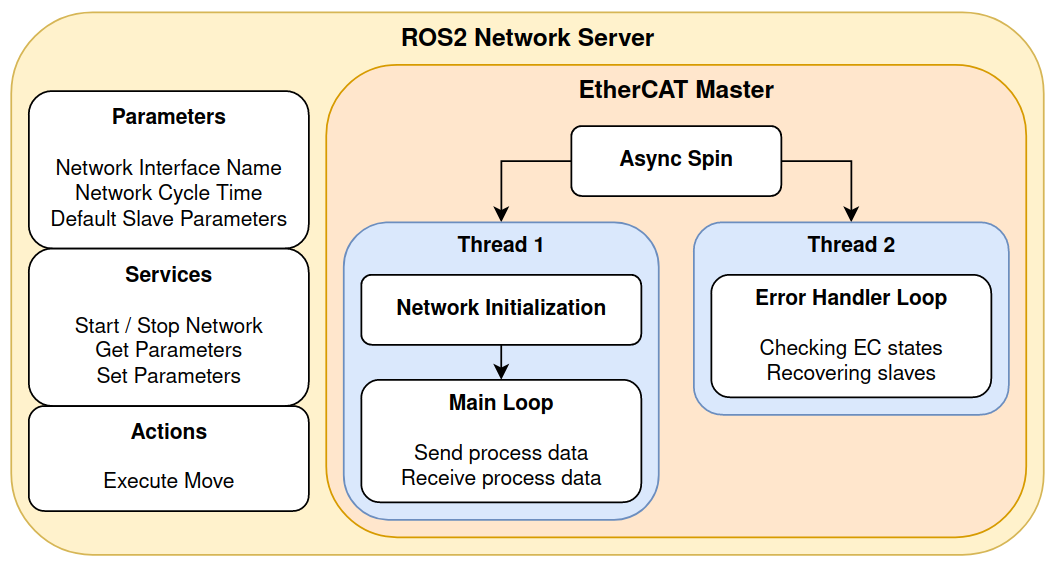
\includegraphics[width=\linewidth]{../resources/figures/ros_ecat_server.png}
	\caption{ROS Network Server}
	\label{fig:ros_ecat_server}
\end{figure}

\lstset{style=cpp}
\begin{lstlisting}[caption=ROS Server Parameters,label=lst:ros_server_parameters]
std::string _network_interface_param{};
uint64_t _network_cycle_period_us_param{};
std::vector<std::pair<uint64_t, std::vector<Parameter>>> _slave_params{};
\end{lstlisting}

\subsection{ROS user interface}

To facilitate user interaction with the functionalities a user interface was developed as a plugin for RQT.
It provides three tabs through which the network is controlled and a fourth for reading direct logging output. 

\subsubsection{Network}

\textcolor{red}{INSERT IMAGE OF UI}

The network tab is meant for detecting and selecting a running ROS Network Server. 
A table view presents the parameters exposed by the selected server, through which the user can edit each parameter and write it to the selected server node. 

\subsubsection{Step response}

\textcolor{red}{INSERT IMAGE OF UI}

The step response tab contains all that is related to the step-type move. 
This includes setting starting and stopping positions, reading and writing slave parameters, and visualizing the data received from the network server feedback. 

The visualization can be selectively chosen to display a variety of plots:
\begin{itemize}
	\item Achieved position / velocity / acceleration
	\item Bode plot
	\item Root locus plot
\end{itemize}

\subsubsection{Frequency response}

\textcolor{red}{INSERT IMAGE OF UI}

The frequency response tab contains all that is related to the sinusoidal type move. 
It allows for movement with two superimposed sine waves, giving control of both frequency and amplitude of each. 

The visualization can be selectively chosen to display a variety of plots.

\begin{itemize}
	\item Achieved position / velocity / acceleration
	\item Amplitude spectrum
	\item Power spectrum
\end{itemize}

Only frequencies below the Nyquist frequency of the network can be visualized.
For the ECT60 controller this means only frequencies up to 1 KHz can be analyzed using this method. 

%%%%%%%%%%%%%%%%%%%%%%%%%%%%%%%%%%%%%%%%%%%%%%%%%%%%%%%%%%%%%%%%%%%%%%%%%%%%%%%%%%%%%%%%%%%%%%%
%%%%%%%%%%%%%%%%%%%%%%%%%%%%%%%%%%%%%%%%%%%%%%%%%%%%%%%%%%%%%%%%%%%%%%%%%%%%%%%%%%%%%%%%%%%%%%%
\subsection{Mechanical setup}

\begin{figure}[H]
	\centering
	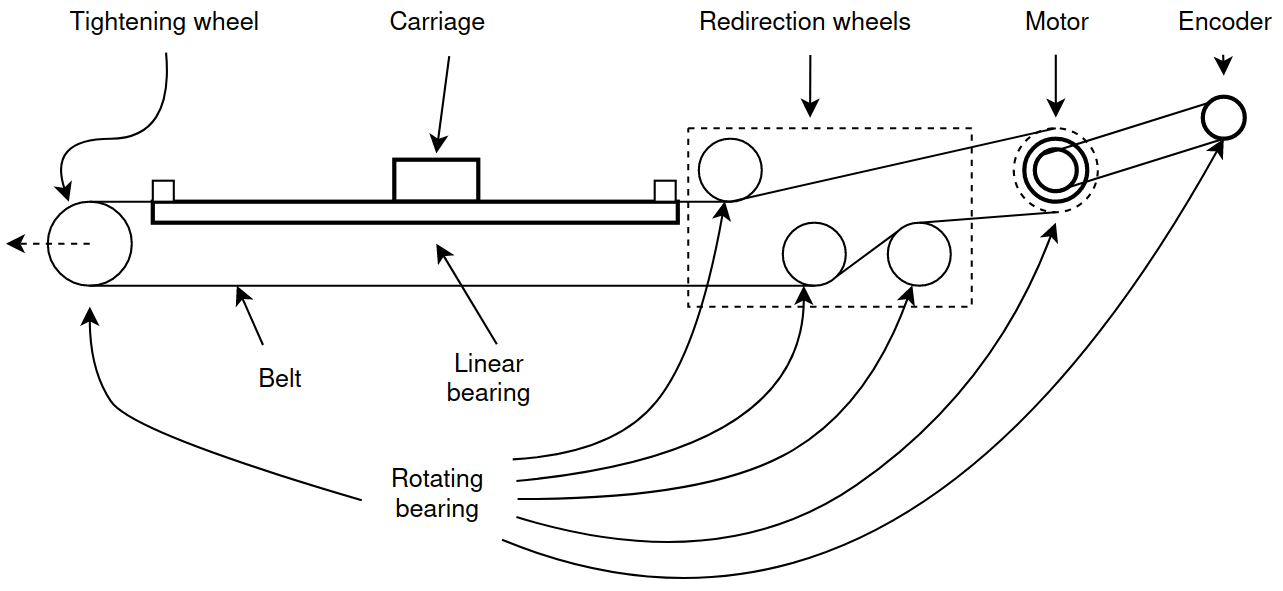
\includegraphics[width=\linewidth]{../resources/figures/mechanical_system.png}
	\caption{System diagram}
	\label{fig:mechanical_system_diagram}
\end{figure}

\begin{figure}[H]
	\centering
	\begin{subfigure}{.5\textwidth}
		\centering
		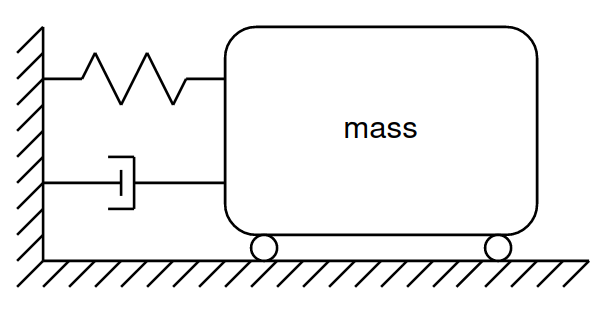
\includegraphics[width=0.7\linewidth]{../resources/figures/spring_damper_diagram.png}
	\end{subfigure}%
	\begin{subfigure}{.5\textwidth}
		\centering
		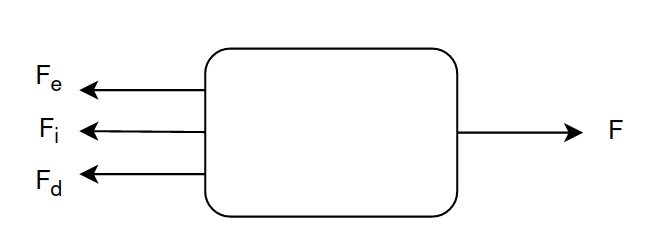
\includegraphics[width=\linewidth]{../resources/figures/free_body_diagram.png}
	\end{subfigure}
	\caption{Free body diagram}
	\label{fig:free_body_diagram}
\end{figure}


Derived equation is a spring-mass-damper system.

\begin{align}
	F_e = & kx \\
	F_i = & m \cdot a = m \dfrac{dv}{dt} = m \dfrac{d^2 x}{d t^2} \\
	F_d = & c \cdot v = c \dfrac{dx}{dt} \\
	0 = & F - F_e - F_i - F_d \\
	0 = & F - kx - m \dfrac{d^2 x}{d t^2} - c \dfrac{dx}{dt} \\
	\dfrac{d^2 x}{d t^2} = & \dfrac{1}{m} \left( F - c \dfrac{dx}{dt} - kx \right) 
\end{align}

Apply Laplace to equation terms

\begin{align}
	\mathcal{L}\left[ \dfrac{d^2 x(t)}{d t^2} \right] = & s^2 X(s) - sx(0) - \dfrac{dx(0)}{dt} \\
	\mathcal{L}\left[ \dfrac{dx(t)}{dt} \right] = & sX(s) - x(0) \\	
	\mathcal{L}\left[ x(t) \right] = & X(s) \\
	\mathcal{L}\left[ F(t) \right] = & F(s) \\
	x(0) = & 0 \\
	\dfrac{dx(0)}{dt} = & 0 \\
	\mathcal{L}\left[ \dfrac{d^2 x(t)}{d t^2} \right] = & s^2 X(s) \\
	\mathcal{L}\left[ \dfrac{dx(t)}{dt} \right] = & sX(s)
\end{align}

Replacing into equations

\begin{align}
	F(s) = & m s^2 X(s) + c s X(s) + k X(s) \\
	F(s) = & X(s) \left( m s^2 + c s + k \right) \\
	H(s) = & \dfrac{X(s)}{F(s)} = \dfrac{1}{m s^2 + c s + k}
\end{align}

Transforming from S to Z domain

\begin{align}
	s = & \dfrac{z - 1}{T_s} \\
	H(z) = & \dfrac{1}{m \left( \dfrac{z - 1}{T_s} \right)^2 + c \dfrac{z - 1}{T_s} + k} \\
	= & \dfrac{1}{ z^2 \dfrac{ k T_s - m }{ T^2_s } + z \dfrac{ c T_s - 2 m }{ T^2 } - \dfrac{c}{T_s} + \dfrac{m}{T^2_s} } \\
	= & \dfrac{1}{ z^2 \left( \dfrac{k}{T_s} - \dfrac{m}{T^2_s} \right) + z \left( \dfrac{c}{T_s} - \dfrac{2m}{T^2_s} \right) - \dfrac{c}{T_s} + \dfrac{m}{T^2_s} }
\end{align}

\begin{tcolorbox}
	The system transfer function can be described by the following equation.
	
	\textcolor{red}{BETTER GET THIS SIMPLE ONE RIGHT}
	
	\begin{align}
	\end{align}
	where $x$ is something, $T_s$ is also something ...
\end{tcolorbox}

%%%%%%%%%%%%%%%%%%%%%%%%%%%%%%%%%%%%%%%%%%%%%%%%%%%%%%%%%%%%%%%%%%%%%%%%%%%%%%%%%%%%%%%%%%%%%%%
%%%%%%%%%%%%%%%%%%%%%%%%%%%%%%%%%%%%%%%%%%%%%%%%%%%%%%%%%%%%%%%%%%%%%%%%%%%%%%%%%%%%%%%%%%%%%%%
\section{Controller setup}

The specific selection of EtherCAT device plays a great role in what setup is possible. 
This is because each manufacturer is free to select any controller implementation. 
The object dictionary entries used for tuning the controller resides outside the standardized dictionary space.

Using the ECT60 selected for this project, the following setup was selected as the default. 
EtherCAT motor controllers can support multiple types of cyclic operational modes. The ECT60 only supports the cyclic position mode. 
It is capable of applying field oriented control on 2-phase stepper motors. 

\textcolor{red}{DESCRIBE THE CYCLIC POSITION MODE PROCESS IMAGE}

\subsection{Control parameters}

As with all EtherCAT devices, a list of control parameters are available as can be seen from the devices object dictionary definition file.

While originally it was intended to develop a method for automatically detecting parameters related to motor control, that is not a possibility. 
Instead the relevant parameters have been manually selected. 

It's because each manufacturer can implement their own controller types without any imposed limitations by EtherCAT standard. 

In cyclic position mode the controller must generate the position profile wanted.
In case of stepped commands, the 0x2022:00 parameter must be set to avoid alarm states when requesting a large move. 

\begin{table}[H]
	\centering
	\begin{tabular}{|c|c|c|c|}
		\hline
		\textbf{Object Address} & \textbf{Variable name} & \textbf{Unit} & \textbf{Default value} \\
		\hline
		0x2009:00 & Filter time constant & $\mu$s & - \\
		\hline
		0x200B:02 & Current loop Kp (proportional gain) & - & - \\
		\hline
		0x200B:03 & Current loop Ki (integral gain) & - & - \\
		\hline
		0x200B:04 & Current loop Kc (controller gain) & - & - \\
		\hline
		0x200C:04 & Motor resistance & mOhm & - \\
		\hline
		0x200C:05 & Motor inductance & mH & - \\
		\hline
		0x200C:06 & Motor back EMF coefficient & - & - \\
		\hline
		0x2022:00 & Position excess alarm value & - & - \\
		\hline
		0x2025:01 & Servo speed filter FV1 & Hz & - \\
		\hline
		0x2025:02 & Servo speed filter FV2 & Hz & - \\
		\hline
		0x2025:03 & Servo speed filter FPOUT & Hz & - \\
		\hline
		0x2026:01 & Servo Mode 2 Kp (proportional gain) & - & - \\
		\hline
		0x2026:02 & Servo Mode 2 Ki (integral gain) & - & - \\
		\hline
		0x2026:03 & Servo Mode 2 Kv1 (velocity feedback gain 1) & - & - \\
		\hline
		0x2026:04 & Servo Mode 2 Kv2 (velocity feedback gain 2) & - & - \\
		\hline
		0x2026:05 & Servo Mode 2 Kvff (velocity feed forward gain) & - & - \\
		\hline
		0x2060:00 & Harmonic resonance filter amplitude & - & - \\
		\hline
		0x2061:00 & Phase A of resonance filter & - & - \\
		\hline
		0x2062:00 & Phase B of resonance filter & - & - \\
		\hline
	\end{tabular}
	\caption{Motor controller parameters}
	\label{tab:controller_parameters}
\end{table}

\subsection{Possible internal controller structure}

Wow, that's a really nice illustration here

Inner loop: Current loop. Takes motor resistance, BEMF, and inductance into calculation. Parameters are Ki, Kc, Kp + resonance filter. 

Mid loop: Velocity loop. Servo speed filter parameters. Feed forward style controller with filters?

Outer loop: Position/Servo loop. Servo Mode 2 parameters. Feed forward style controller + filter integration time.

\textcolor{red}{CREATE EACH LOOP AS MASSIVE FIGURE FROM SIMULINK}

\subsection{Possible transfer function}

Hmm, this is a larger thing ...

\textcolor{red}{DERIVE FROM THE PROPOSED CONTROLLER ABOVE}

\subsection{Tuning strategy}

Determine motor resistance, inductance, and back EMF experimentally or from datasheet. 

The inner loop should be tuned while motor is connected to an oscilloscope. Smooth current waveforms when driving constant velocity steady state. 

\begin{table}[H]
	\centering
	\begin{tabular}{|c|c|c|}
		\hline
		\textbf{Parameter} & \textbf{Increase} & \textbf{Decrease} \\
		\hline
		Kp &  &  \\
		\hline
		Ki &  &  \\
		\hline
		Kc &  &  \\
		\hline
	\end{tabular}
	\caption{Inner loop tuning}
	\label{tab:controller_tuning_inner}
\end{table}

The servo loop is tunable from the position feedback. 

\begin{table}[H]
	\centering
	\begin{tabular}{|c|c|c|}
		\hline
		\textbf{Parameter} & \textbf{Increase} & \textbf{Decrease} \\
		\hline
		Kp &  & \\
		\hline
		Ki &  & \\
		\hline
		Kv1 &  & \\
		\hline
		Kv2 &  & \\
		\hline
		Kvff &  & \\
		\hline
		FV1 &  & \\
		\hline
		FV2 &  & \\
		\hline
		FPOUT &  & \\
		\hline
		Filter time constant &  & \\
		\hline
	\end{tabular}
	\caption{Servo loop tuning}
	\label{tab:controller_tuning_servo}
\end{table}

Reducing the vibrations is done by ear, as it is not possible to diagnose using the position feedback. 
The position feedback is much too slow. 

\begin{table}[H]
	\centering
	\begin{tabular}{|c|c|c|}
		\hline
		\textbf{Parameter} & \textbf{Increase} & \textbf{Decrease} \\
		\hline
		Harmonic resonance filter amplitude &  & \\
		\hline
		Resonance filter Phase A &  & \\
		\hline
		Resonance filter Phase B &  & \\
		\hline
	\end{tabular}
	\caption{Vibration tuning}
	\label{tab:controller_tuning_vibration}
\end{table}

%%%%%%%%%%%%%%%%%%%%%%%%%%%%%%%%%%%%%%%%%%%%%%%%%%%%%%%%%%%%%%%%%%%%%%%%%%%%%%%%%%%%%%%%%%%%%%%
%%%%%%%%%%%%%%%%%%%%%%%%%%%%%%%%%%%%%%%%%%%%%%%%%%%%%%%%%%%%%%%%%%%%%%%%%%%%%%%%%%%%%%%%%%%%%%%
\section{System identification}

To achieve system identification, the resulting data from an executed step response move is transformed using Z-transform.
This directly provides the transfer function which can then be further analyzed. 

To help the user, a set of plots are also provided, root locus, other good shit.

While originally the tuning was intended to be algorithmic and automatic, it isn't.
Ordering of tuning parameters, inner outer loops, differences specific to this device. 

\begin{itemize}
	\item Execute step move
	\item Normalize feedback
	\item Z-transform
	\item Data presentation
	\item Parameter adjustment order? 
\end{itemize}

\subsection{Step execution}

Setting the allowable position deviation to a value above the requested step size. 
Running the move and recording feedback and requested values. 
Transforming the discrete data using Matlab to determine poles and zeros. 
Input poles and zeros into UI and plotting. 

\textcolor{red}{INSERT SOME CODE}
\lstset{style=python}
\begin{lstlisting}[language=python]
\end{lstlisting}

\subsection{Transfer function estimation}

Determining a transfer function from the generated discrete data-set is done using the MATLAB System Identification toolbox. 
Some algorithm should be written for this to integrate it into the UI as the toolbox functions cannot be exported using MATLAB Coder. 

\textcolor{red}{INSERT CODE USED FOR PLOT GENERATION}
\lstset{style=matlab}
\begin{lstlisting}[language=matlab]
\end{lstlisting}

\subsection{Data presentation}

\subsubsection{Step and impulse response}

Step response is simply graphing the position data. 
Impulse response is calculated by derivative. 

Graphing it against the estimated transfer function can help determine if the estimation is reasonable. 

\textcolor{red}{INSERT CODE USED FOR PLOT GENERATION}
\lstset{style=python}
\begin{lstlisting}[language=python]
\end{lstlisting}

\subsubsection{Bode}

Bode plot using magnitude and phase. 

Once the transfer function is estimated in the s-space it can be plotted easily.

\textcolor{red}{INSERT CODE USED FOR PLOT GENERATION}
\lstset{style=python}
\begin{lstlisting}[language=python]
\end{lstlisting}

\subsubsection{Root locus}

Root locus from just placing poles and zeros in a rectangular plot

\textcolor{red}{INSERT CODE USED FOR PLOT GENERATION}
\lstset{style=python}
\begin{lstlisting}[language=python]
\end{lstlisting}

%%%%%%%%%%%%%%%%%%%%%%%%%%%%%%%%%%%%%%%%%%%%%%%%%%%%%%%%%%%%%%%%%%%%%%%%%%%%%%%%%%%%%%%%%%%%%%%
%%%%%%%%%%%%%%%%%%%%%%%%%%%%%%%%%%%%%%%%%%%%%%%%%%%%%%%%%%%%%%%%%%%%%%%%%%%%%%%%%%%%%%%%%%%%%%%
\section{Vibration analysis}

Another important factor in reliable motor control is to minimize the level of unwanted vibrations in the system.
This analysis is done by Fourier transforming the result of a sinusoidal move. Various dampening control parameters can then be tuned manually until the spectrum is satisfactory. 

\begin{itemize}
	\item Execute sine for excitation
	\item Discrete Fourier transform
	\item Data presentation
\end{itemize}

\begin{align}
	F_k = & \sum_{n=0}^{N-1} f_n e^{-i 2 \pi k n / N}
\end{align}

\subsection{Sine execution}
\subsection{Discrete Fourier transform}
\subsection{Sampling time constraints}
\subsection{Data presentation}
\subsubsection{Spectrum plots}

\textcolor{red}{INSERT CODE USED FOR PLOT GENERATION}
\lstset{style=python}
\begin{lstlisting}[language=python]
\end{lstlisting}


